\chapter{Discussion, Future Work and Conclusion}
\section{Discussion}
Vulture has shown that word-gesture keyboards are beneficial to mid-air text-entry by surpassing earlier work and reaching a text-entry rate of 28 WPM; however, it utilizes pinching as a means of word separation \cite{ref_vulture}. This study aimed to find alternative solutions to word separation and interaction with mid-air, word-gesture keyboards. Rather than pinching or inconvenient glove-use, this study utilized the 3rd-Dimension as well as a bimodal approach.

This study suffered from some of the same issues that were experienced in Vulture, text-entry rates were much slower for mid-air keyboards than the touch-based keyboard. One reason for this was that participants were required to recouple the gestures in motor space with those on the display \cite{ref_vulture}. This affect was described in detail for many of the results in Chapter~\ref{5_results}. Another reason, as seen in Vulture and in other studies \cite{ref_vulture,ref_visual_feedback_focus}, participants heavily rely on the displayed feedback. This was seen mostly due to the small latency introduced when using the Leap Motion to track and display hand motions on the screen. Some participants commented having to slow down to ensure the display more accurately represented their hand movements. If movements were made that were too fast, the visual display would slightly lag behind and so some participants had a tendency to overshoot letters. A final reason, like in Vulture, was that many of the alternatives add to the complexity of text-entry by the forcing explicit delimiting of words. 

\subsection{Pinching Interaction}
This study attempted a pinching method using the Leap Motion in order to have a metric for comparison against Vulture's pinching since this study used a pseudo-implementation of word-gesturing that lacked word-recognition. The text-entry rate for pinching with a single session was 11.3 WPM which was consistent with the mean text-entry rate using Vulture ($M = 11.8$ WPM) for a single session \cite{ref_vulture}. This gave a solid measure for alternative solutions to compare against.

\subsection{3-Dimensional Interaction}
This study showed initial text-entry rates for utilizing the 3rd-Dimension as a means of word separation at 8.6 WPM for the Static-Air approach and 9.6 WPM for the Predictive-Air approach. These approaches underperformed because of the difficulty in mentally coupling word-gestures in motor space with those displayed on the screen with the added factor of having to move in the 3rd-Dimension and interact with an invisible plane to delimit words.

The Predictive-Air Keyboard was not significantly worse than the Pinch-Air Keyboard and needs to be investigated further with a repeated-measures, multiple session study. Both the Static-Air and Predictive-Air suffered from an issue referred to as ``skimming'', demonstrated in Figure~\ref{skimming_problem}. The ``skimming'' issue was when a participant reaches towards the interaction plane and simulates a touch but as they move their hand during the gesturing motion, natural arcing of the participant's hand causes them to lose the simulated touch. The natural arcing motion of the participants also seemed to cause a lot of errors after finishing writing a word because participants would pull their hand back in an arcing motion, especially if their elbow was rested. This would cause their finger to hit the key above the current key they were on and count it as a press, as seen in Figure~\ref{arcing_motion}.

\begin{figure}[h]
	\centering
	\begin{minipage}[t]{2.5in}
		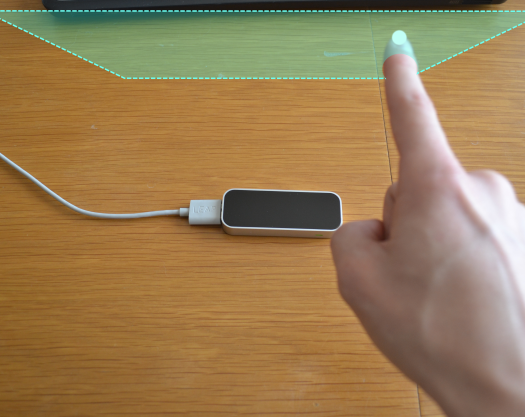
\includegraphics[width=2.5in]{fig_skimming_before}
		\subcaption{Pressing Key}
	\end{minipage}
	\begin{minipage}[t]{2.5in}
		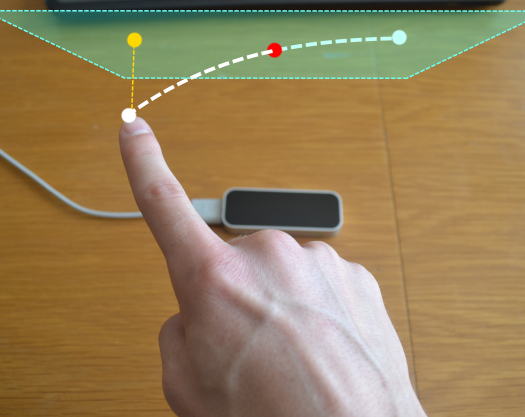
\includegraphics[width=2.5in]{fig_skimming_after}
		\subcaption{Moving to next Letter across Keyboard}
	\end{minipage}
	\caption[Skimming Problem]{Example of how the natural arcing motion of the arm loses touch as moving across the interaction plane. \textbf{(a)} shows the user pressing a key. \textbf{(b)} shows the intended destination \textbf{yellow} and the accidental release \textbf{red}.}
	\label{skimming_problem}
\end{figure}

It's very interesting to note that the Static-Air implementation was used to project a mid-air keyboard onto flat surfaces, simulating a touch screen. This was the Leap Surface Keyboard. The Leap Surface was essentially indistinguishable from the Touch Screen Keyboard in terms of performance and text-entry rate, reaching 17.1 WPM for a single session. The Leap Surface Keyboard handily proves how essential it is to avoid having a decoupled motor space and display space. This hints that the Static-Air Keyboard may substantially benefit from an input plane displayed using augmented reality.

\subsection{Bimodal Interaction}
Bimodal mid-air interactions were shown to be very promising in this study and it should be noted that any other secondary input could be used as the source for touch simulation. The Bimodal-Air Keyboard reached a text-entry rate of 15.8 WPM for a single session which was a significant improvement over using pinching or utilizing the 3rd-Dimension. The Bimodal-Air Keyboard was also often times indistinguishable from the Touch Screen Keyboard for many other dependent measures, detailed in Chapter~\ref{5_results}. The Bimodal-Air keyboard needs to be further investigated in a repeated-measures, multiple session study on a word-gesture keyboard implemented with word-recognition.

The Bimodal-Air was not without some of its own drawbacks. As with the other mid-air keyboards that were implemented with the Leap Motion, there was an associated input plane that the gestures were projected onto as the participant' moved their hands. This plane, if calibrated or oriented incorrectly, could lead to higher error rates and less precision overall.

\subsection{Lacking Word-Recognition}
There were some glaring limitations to using a pseudo-implementation of word-gesturing as opposed to using a full word-recognition implementation. A major differences was that the pseudo-implementation analyzed the gesture as it was being created, showing participants real-time updates of what was happening to the path they were creating. As the gesture was being created, the system attempted to guess the current character being pressed based on the deviations in the gesture and then compared those deviations with the current characters that the participant was trying to achieve and against the previously detected deviation. The limitation that this imposes, seeing real-time character-level updates, was that most participants would interrupt their current word-gesture in order to fix the errors being created mid-gesture which is unnatural for word-gesturing. As well, the fidelity for making errors was much higher which allowed these interruptions to sometimes occur frequently. The lack of word-recognition means that words that were not present in any dictionary could be produced through gesturing which again was counter-intuitive. Also once a mistake was made, the likelihood to see more errors increased because the path protection would be disabled.

\section{Future Work}
There were many things to consider when looking at improvements to be made or additional studies that could be conducted.

\subsection{Implement Word-Recognition}
The most important change to this study that needs to be explored is to re-conduct the study using a standardized word-gesture keyboard implementation with word-recognition. This single improvement will give better and more standardized results across the board. There would also be no need for any modified variables, and less error measures could have been observed. There should also be an increase in text-entry rates since participants would not be distracted with errors mid-gesture.

\subsection{Redesign Task}
The task for the study needs to be substantially redesigned to fit a word-recognition implementation of the word-gesture keyboards. First, the trials need to be phrases instead of single words to better track text-entry and error rates. Next, there should not be any requirement to fix words, it should just feel natural for the participant and they can fix errors where they feel it is necessary. Finally, the number of trials needs to be increased by a significant amount and the study needs to be designed for repeated sessions so that improvements in text-entry rate can be seen. With repeated sessions and actual word-recognition, the Bimodal-Air keyboard is expected to achieve text-entry rates superior to those found in Vulture.

\subsection{Augmented Reality}
In an effort to decrease the mental coupling required between the gesture motor-space and the keyboard display, augmented reality would be a huge boon for 3-Dimensional mid-air implementations. This is theorized to benefit the Static-Air Keyboard the most due to the success of the Leap Surface Keyboard which is just the Static-Air keyboard projected onto a surface. Participants being able to directly see the mid-air keyboard they are using would be expected to substantially increase text-entry rates.

\subsection{The ``Skimming'' Issue}
As a first thought to solve the ``skimming'' issue, there is a seemingly obvious solution to the problem. Simply, as shown in Figure~\ref{skimming_problem_fix}, once a simulated touch has been made, increase the interaction plane's threshold in the participant's direction enough so that the participant's hand doesn't leave the surface when moving from side to side or up and down. This change should see improved results for the Static-Air Keyboard since there would be many less times where the user accidentally exits the interaction plane. A similar approach could also be used for the Predictive-Air because sometimes quick side to side movements were seen as a touch being released.

\begin{figure}[h]
	\centering
	\begin{minipage}[t]{2.5in}
		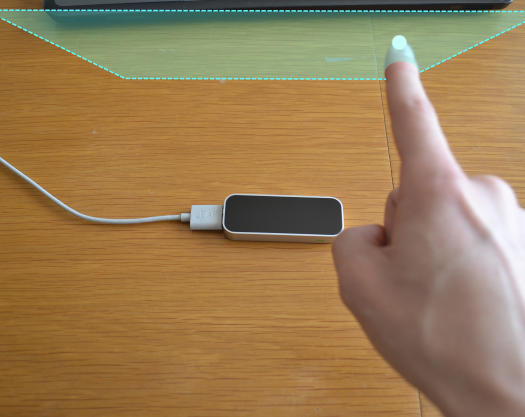
\includegraphics[width=2.5in]{fig_skimming_fix_before}
		\subcaption{Intersecting Plane to hit First Key}
	\end{minipage}
	\begin{minipage}[t]{2.5in}
		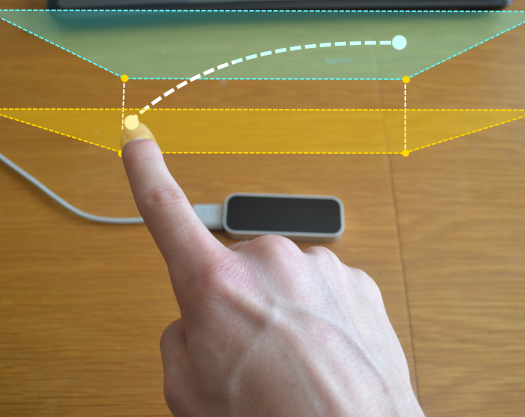
\includegraphics[width=2.5in]{fig_skimming_fix_after}
		\subcaption{Increased Release Threshold}
	\end{minipage}
	\caption[``Skimming Solution'']{An example of how the ``skimming'' issue could be fixed by increasing the release threshold after touching. \textbf{(a)} shows the user pressing the first key. \textbf{(b)} shows the increased release threshold for the interaction plane as the user moves across to the next key.}
	\label{skimming_problem_fix}
\end{figure}

\subsection{Better Tracking}
A simple observation that was made by the researcher was that there were many times that the Leap Motion had issues detecting participants' pointer fingers or palms. A major factor of these detection issues was due to the positioning of the Leap Motion Controller itself, as well as some participants holding their hand in an upward position, like shown in Figure~\ref{finger_blocked}. A simple solution to this issue is to angle the leap so that it is facing the participant at a better angle, as seen in Figure~\ref{finger_seen}.

\begin{figure}[h]
	\centering
	\begin{minipage}[t]{2.5in}
		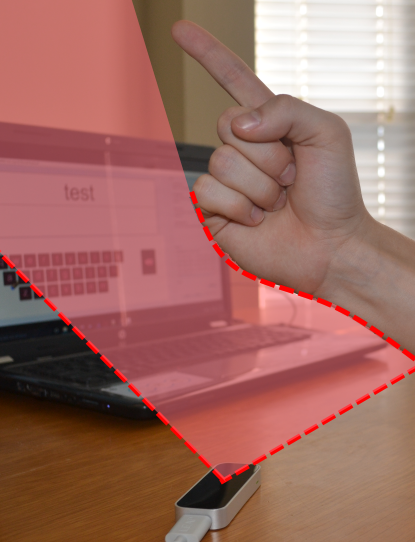
\includegraphics[width=2.5in]{fig_blocking}
		\subcaption{Hand Blocking Finger}
		\label{finger_blocked}
	\end{minipage}
	\begin{minipage}[t]{2.5in}
		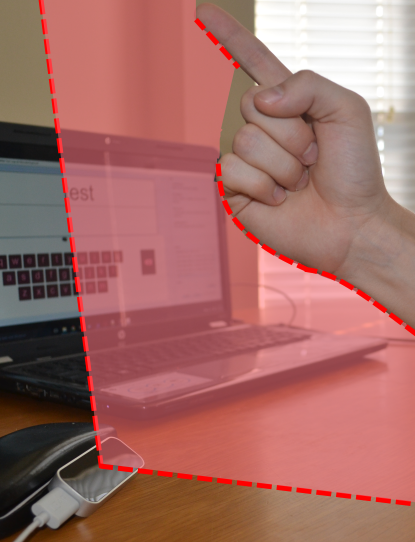
\includegraphics[width=2.5in]{fig_angled}
		\subcaption{Angle Reveals Finger}
		\label{finger_seen}
	\end{minipage}
	\caption[Blocking Problem]{Examples of how some participants blocked their finger from being tracked. \textbf{(a)} shows the user blocking the view of their finger with their hand. \textbf{(b)} shows how an angled Leap Motion Controller might solve the problem.}
	\label{blocking problem}
\end{figure}

\subsection{Alternative Interaction Plane}
Something that was observed with all mid-air keyboards was that as the participants moved across the interaction plane, sometimes the side-to-side movements and up and down movements were not represented as expected, as seen in Figure~\ref{bad_calib_problem}. Better approaches to calibration and plane-creation need to be used such as those used and mentioned in Personal Space and like methods \cite{ref_alvin_thesis,ref_darren_thesis}. A spherical or even curved interaction plane designed for each individual participant would greatly benefit all of the mid-air keyboards especially so that participants would be able to rest their arms. With a flat, quadrilateral plane, many participants suffered the same issues as mentioned in \cite{ref_alvin_thesis}, especially when moving to the extreme edges of the projected keyboard.

\begin{figure}[h]
	\centering
	\begin{minipage}[t]{6in}
		\begin{minipage}[t]{1.5in}
			\begin{minipage}[t]{1.5in}
				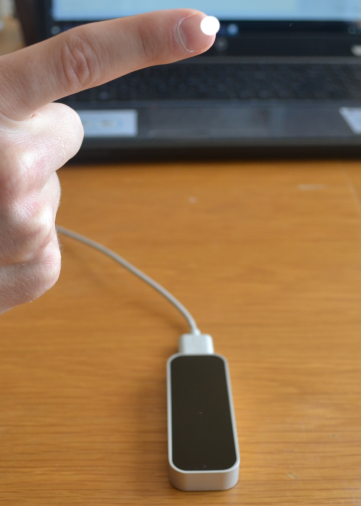
\includegraphics[width=1.5in]{fig_bad_calib_before}
			\end{minipage}
			
			\begin{minipage}[t]{1.5in}
				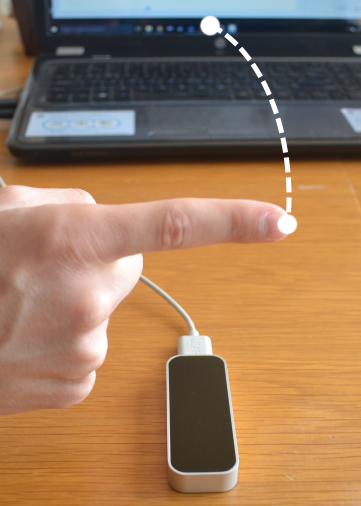
\includegraphics[width=1.5in]{fig_bad_calib_after}
			\end{minipage}
			\subcaption{Movement}
		\end{minipage}
		\begin{minipage}[t]{4.5in}
			\begin{minipage}[t]{4.3in}
				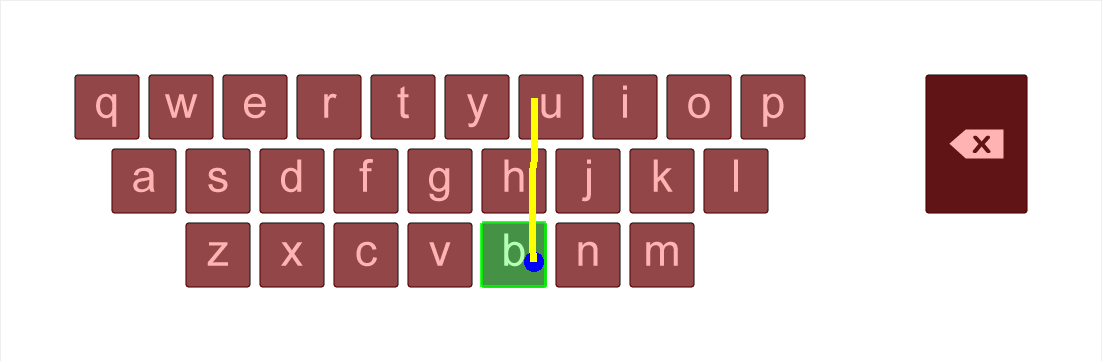
\includegraphics[width=4in]{fig_intended_path}
			\end{minipage}
			
			\begin{minipage}[t]{4.3in}
				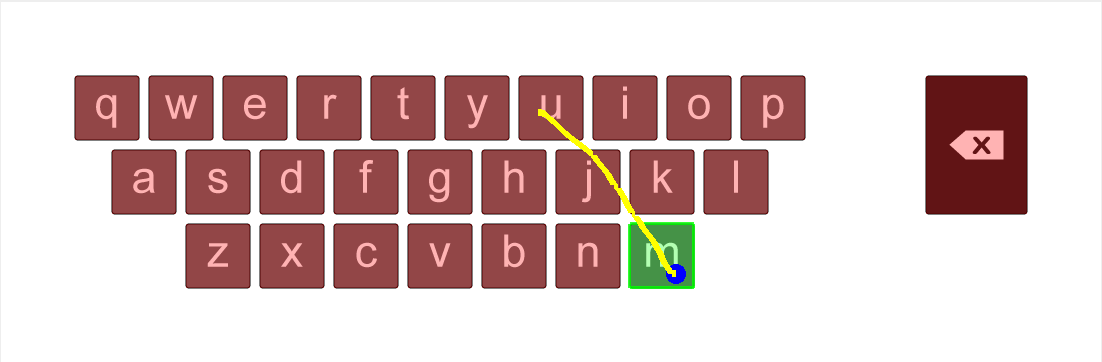
\includegraphics[width=4in]{fig_actual_path}
			\end{minipage}
			\subcaption{Intended Path \textbf{Top} vs. Actual Path \textbf{Bottom}}
		\end{minipage}
	\end{minipage}
	\caption[Bad Calibration Example]{Example showing how a bad calibration affects movement. \textbf{(a)} shows a user trying to make a vertical movement. \textbf{(b)} shows how the actual path was misaligned because of the calibration and orientation of the Leap Motion Controller.}
	\label{bad_calib_problem}
\end{figure}

\subsection{Multi-functional Space}
Utilizing the 3rd-Dimension for mid-air word-gesturing keyboards, when not touching the interaction plane to simulate touch, hand gestures could be used to control a cursor or for other gestures. This would allow users to fully interact with screens of any kind, including projections, and not limit the user to a keyboard and mouse.

\subsection{Image Processing}
After using the Leap Surface Keyboard and projecting a virtual keyboard over just a printed sheet, an addition that could be added to make the feature much more versatile is image processing. Being able to print and use any keyboard for word gesturing or otherwise could be interesting and highly beneficial.

\subsection{Gaming Console Keyboards} \label{future_gaming_keyboard}
An afterthought, from using the Xbox Controller Keyboard in the pre-pilot and the pilot study, is that it would be very beneficial to apply what has been learned from this study and word-gesturing in general to gaming console keyboards. There are two options for implementing a word-gesture keyboard for gaming consoles. The first is to implement a mid-air word-gesture keyboard using the Xbox Kinect or using the Wii Remotes. The second option would be to transition from the standard console keyboards to a word-gesture keyboard just using standard console controllers. The word-gesture keyboard would most likely have to be bimodal. The user would hold the 'A' button while simulating touch and use the thumb stick to move a cursor around for word-gesturing. Either method would be a great improvement over single character text-entry currently seen on modern gaming consoles.

\subsection{Accessibility}
A major motivation for this research was the idea of applying it for amputees or those with disabilities that affect their performance using a standard keyboard. A proper study in accessibility should be performed to utilize the Bimodal-Air keyboard for users with disabilities.

\section {Conclusion}
Word-gesture keyboards show a promising means to efficient, mid-air text-entry by tracing word-gestures instead of slow, single-input text-entry \cite{ref_vulture}. This study demonstrated alternative ways to delimit the separation of words for mid-air, word-gesture keyboards. It was shown that utilizing the 3rd-Dimension as a means of word separation is too complex to be beneficial when paired with a decoupled gesture-space and keyboard display. As demonstrated by projecting a Static-Air plane onto a surface with the Leap Surface Keyboard, better results may be achieved when using the 3rd-Dimension as a means of word-separation if they are complimented by an augmented reality design to recouple the gesture-space and keyboard display. Another method to lessen the severity of a decoupled gesture-space and keyboard display is that the interaction plane needs to use new techniques to be better calibrated for each individual user and to display more accurate results and control \cite{ref_alvin_thesis,ref_darren_thesis}. Finally, the empirical results from this study shows that using a bimodal technique as a means of word separation would greatly benefit mid-air, word-gesture keyboards. The Bimodal-Air keyboard was slower in text-entry rates than the Touch Screen Keyboard; however, the bimodal method was near indistinguishable from the touch screen for almost all other empirical results and was also better than pinching for nearly all results. This study needs to have a follow-up study with redesigned trials using a full word-gesture keyboard implementation with repeated measures and reoccurring sessions to further investigate bimodal techniques for mid-air text-entry. A bimodal approach just might be the future of mid-air text-entry for word-gesture keyboards.